\section{Maxwell Gleichungen}
\subsection{Maxwell Gleichungen}
\begin{longtable}{|p{.08\textwidth}|p{.25\textwidth} |p{.25\textwidth}|p{.30\textwidth}| }
	\hline
	\textbf{Gesetz}&\textbf{Differentialform} &\textbf{Differentialform} &\textbf{Integralform}\\
	&1. Art & 2. Art &\\
	\hline
	1.&$\divergenz \vec{D}=\nabla \cdot \vec{D}= \rho$ & $\divergenz \vec{E}= \frac{\rho}{\epsilon}$&$\oint\limits_{\partial V}\vec{D}\cdot d\vec{A}=\int\int\int\limits_{V}\rho \cdot dV=Q$\\
	\hline
	2.&$\divergenz \vec{B}=\nabla \cdot \vec{B}=0$&$\divergenz \vec{H}=\nabla \cdot \vec{H}=0 $&$\oint\limits_{\partial V}\vec{B}\cdot d\vec{A}=0$\\
	\hline
	3.&$\rotation \vec{E}=\nabla \times \vec{E}=-\frac{\partial B}{\partial t}$&$\rotation \vec{E}=\nabla \times \vec{E}=-\mu \frac{\partial H}{\partial t}$&$\oint\limits_{\partial A}\vec{E}\cdot ds=-\iint\limits_{A}\frac{\partial B}{\partial t}\cdot dA$\\
	\hline
	4.&$\rotation\vec{B}=\nabla\times\vec{B}=\mu_0 (J+\frac{\partial D}{\partial t})$&$\rotation \vec{H}=\nabla \times \vec{H}=\sigma\vec{E}+\epsilon \frac{\partial E}{\partial t}$&$\oint\limits_{\partial A} \vec{H}\cdot ds$\\
	\hline
\end{longtable}
\subsection{Erstes Maxwell-Gesetz}
Gausssches Gesetz für Elektrische Felder\\
\begin{tabular}{p{.45\textwidth} p{.45\textwidth}}
	\textbf{Differentialform}&\textbf{Integralform}\\
	Das E-Feld ist ein Quellenfeld. Die Ladung ist die Quelle des elektrischen Feldes. & Der elektrische Fuss durch die geschlossene Oberfläche eines Volumen ist direkt proportional zur elektrischen Ladung in seinem inneren. \\
\end{tabular}
\subsection{Zweites Maxwell-Gesetz}
Gausssches Gesetz für Magnetische Felder\\
\begin{tabular}{p{.45\textwidth} p{.45\textwidth}}
	\textbf{Differentialform}&\textbf{Integralform}\\
	Das B-Feld ist quellenfrei. Es gibt keine magnetische Monopole (Magnet welcher nur ein Pol hat).& Der magnetische Fluss durch die Oberfläche eines Volumen ist gleich der magnetischen Ladung in seinem inneren, nämlich Null.\\
\end{tabular}
\subsection{Drittes Maxwell-Gesetz}
Induktionsgesetz\\
\begin{tabular}{p{.45\textwidth} p{.45\textwidth}}
	\textbf{Differentialform}&\textbf{Integralform}\\
	Jede Änderung des B-Feldes führt zu einem elektrischen Gegenfeld. Die Wirbel des elektrischen Feldes sind von der zeitlichen Änderung der magnetischen Flussdichte abhängig (Induktionsgesetz). & Die elektrische Zirkulation (Umlaufintegral eines Vektorfeldes über  einen geschlossenen Weg) über eine Kurve einer Fläche ist gleich der negativen Änderung des magnetischen Flusses durch die Fläche.\\
\end{tabular}
\subsection{Viertes Maxwell-Gesetz}
Durchflutungsgesetz\\
\begin{tabular}{p{.45\textwidth} p{.45\textwidth}}
	\textbf{Differentialform}&\textbf{Integralform}\\
	Die Wirbel des Magnetfeldes hängen von der Stromdichte und von der elektrischen Flussdichte ab. Die zeitliche Änderung der Flussdichte wird als Verschiebungsstromdichte bezeichnet (Durchflutungsgesetz)& Die magnetische Zirkulation über eine Kurve einer Fläche ist gleich der Summe aus dem Leitungsstrom und der zeitlichen Änderung des Flusses durch die Fläche. \\
\end{tabular}
\clearpage
\pagebreak

\subsection{Elektromagnetische Wellengleichung}
Eine Elektromagnetische Welle erfüllt immer die nachfolgenden Gleichung. Anhand dieser ist ersichtlich das für die Welle keine Ladung nötig ist sonder das E-Feld und das B-Feld beschäftigen sich mit sich selber und weil ein E-Feld und B-Feld nach sich zieht und umgekehrt. Damit breitet sich die Welle aus. \\
\begin{minipage}{8cm}
	\[\begin{matrix}
	\divergenz \vec{E}=0\\
	\divergenz \vec{B}=0\\
	\rotation \vec{H}=\epsilon_{0}\mu_{0} \frac{\partial \vec{E}}{\partial t}\\
	\rotation \vec{B}=-\dfrac{\partial \vec{B}}{\partial t}\\
	\rotation \vec{E}=-\mu_{0}\dfrac{\partial \vec{H}}{\partial t}
	\end{matrix}\]
\end{minipage}
\begin{minipage}{8cm}
	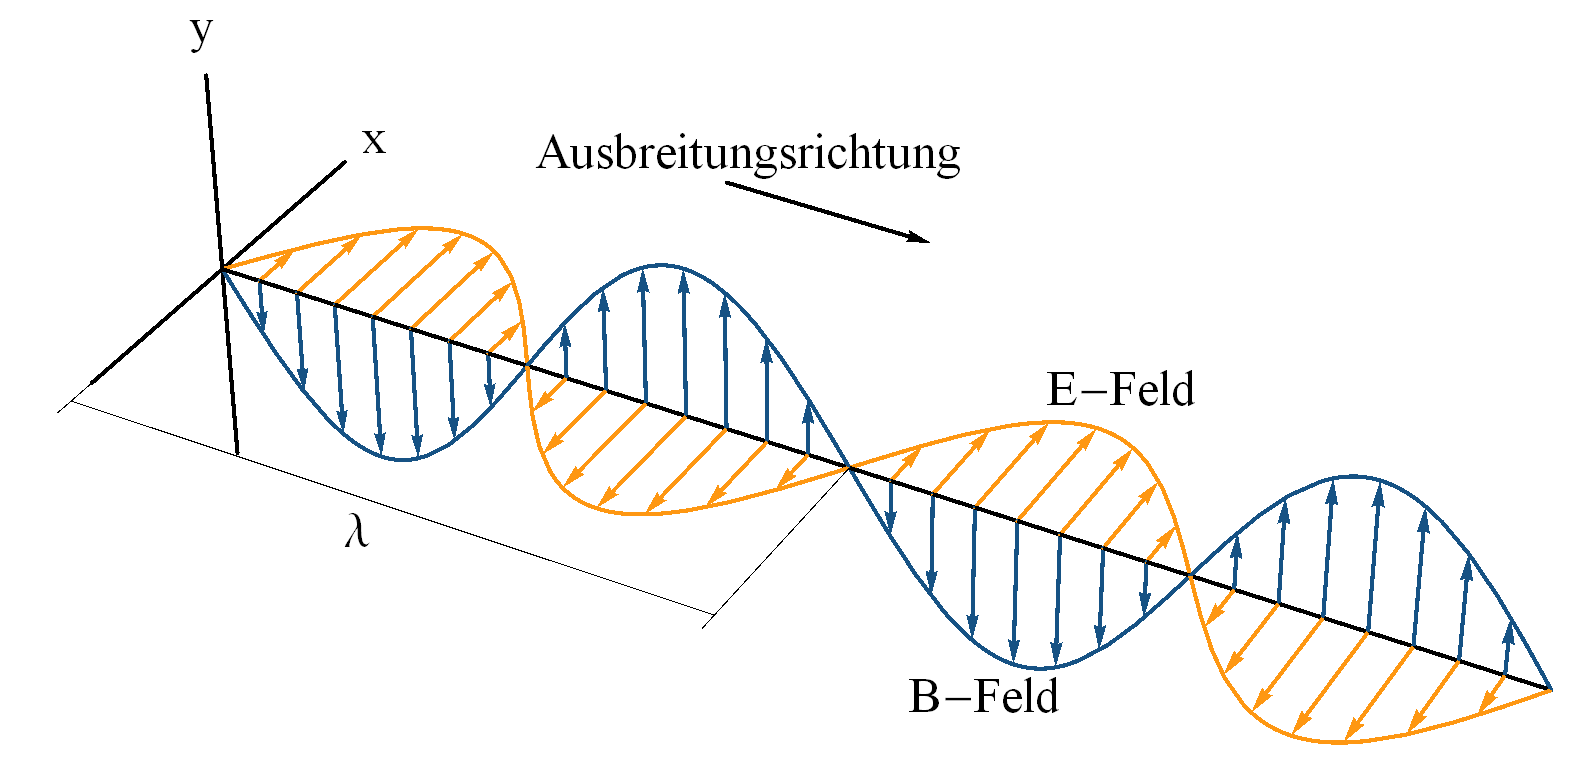
\includegraphics[width=8cm]{images/EMWelle.jpg}
\end{minipage}

\begin{tabular}{p{.45\textwidth} p{.45\textwidth}}
	{\hspace{-2.5cm}\centering\textbf{Magnetisches Feld}\par}&{\hspace{-2.5cm}\centering\textbf{Elektrisches Feld}\par}\\[-1.5cm]
	\[\Delta\vec{H}-\mu\sigma\frac{\partial \vec{H}}{\partial t}-\mu\epsilon\frac{\partial^{2}\vec{H}}{\partial t^{2}}=0\]&	\[\Delta\vec{E}-\mu\sigma\frac{\partial \vec{E}}{\partial t}-\mu\epsilon\frac{\partial^{2}\vec{E}}{\partial t^{2}}=0\]  \\
\end{tabular}
\subsection{Randbedingungen}
\begin{itemize}
	\item Am Rand zwischen zwei Materialien $H_{t1}=H_{t2}$
	\item Am Rand zwischen zwei Materialien $B_{n1}=B_{n2}$
	\item Am Rand zwischen zwei Materialien $E_{t1}=E_{t2}$
	\item Am Rand zwischen zwei Materialien $D_{n1}=D_{n2}$
\end{itemize}
\subsection{Randwertproblem}
\begin{minipage}{9cm}
	\begin{itemize}
		\item Zeitbereich: $\Delta\vec{H}-\mu\sigma\frac{\partial \vec{H}}{\partial t}-\mu\epsilon\frac{\partial^{2}\vec{H}}{\partial t^{2}}=0$
		\item Frequenzbereich: $\Delta \vec{H}-\imaginär\omega\mu\sigma\vec{H}+\omega^{2}\mu\epsilon\vec{H}=0$
		\item Sobald eine Welle auf einen Rand trifft wird immer ein Teil reflektiert und der andere geht durch
	\end{itemize}	
\end{minipage}
\begin{minipage}{8cm}
	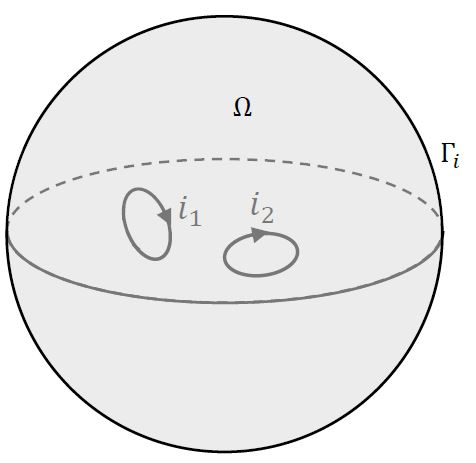
\includegraphics[width=4cm]{images/Randwertproblem.jpg}
\end{minipage}
\subsection{Vorgehen}
	\begin{enumerate}
		\item Partielle Differentialgleichung 2. Ordnung der Welle aufstellen (Elektrisch oder Magnetisch)
		\item In Frequenzbereich transformieren (Annahme sinusförmige Anregung)
		\subitem $\dfrac{\partial \vec{F}}{\partial t}= j\omega F $
		\item Differentialgleichung vereinfachen
		\item Aufstellen der Randbedingungen
		\subitem Randwerte für E-Feld und H-Feld
		\item Wellengleichung mittels Charakteristischem Polynom lösen da Homogen
		\item Bestimmung der Unbekannten Amplituden mittels den Randbedingungen
	\end{enumerate}
\clearpage
\pagebreak
\subsection{Grundlagen zu den Maxwellgleichungen}
Die Maxwell Gleichungen beschreiben, dass die Feldlinien eines sich ändernden Magnetfeldes von ringförmigen elektrischen Feldlinien umgeben sind, auch ohne Vorhandensein von elektrischen Leitern. Darauf die Theorie der elektromagnetischen Wellen auf. Grundlage der Maxwellschen Theorie sind die Maxwellschen Gleichungen. Es zeigt sich, dass die Lösungen der Gleichungen elektromagnetische Wellen beschreiben.\\
\vspace{0.2cm}\\
\renewcommand{\arraystretch}{1.2}
\begin{tabular}{|p{.45\textwidth} |p{.45\textwidth}|}
	\hline
	\textbf{Elektrische Kraft}\newline
	\[\vec{F}=q\cdot \vec{E}\]&
	\textbf{Magnetische Kraft}\newline
	\[\vec{F}=q\cdot(\vec{v}\times \vec{B})\]\\
	\hline
	\textbf{Elektrische Raumladungsdichte}\newline
	Sagt aus wieviel Ladung sich im Raum befindet\newline
	\[ \rho  = \frac{Q}{V}\]&
	\textbf{Elektrische Stromdichte}\newline
	Sagt aus wie die Ladung rämumlich verteilt ist\newline
	\[\vec{J}=\rho \cdot \vec{v}\]\\
	\hline
	\textbf{Wellenimpedanz der Luft}\newline
	\[Z_{0}=\sqrt{\frac{\mu_{0}}{\epsilon_{0}}} \]&
	\textbf{Wellenimpedanz eines Isolators}\newline
	\[Z=\sqrt{\frac{\mu_{0}}{\epsilon}} \]\\
	\hline
	\textbf{Kapazität}\newline
	\[C=\frac{Q}{U} \] &
	\textbf{Induktivität}\newline
	\[L=\frac{N\cdot \Phi }{I} \]\\
	\hline
	\textbf{Magnetische Energie}\newline
	\[W= \frac{1}{2}\cdot L \cdot I^{2}\]&
	\textbf{Elektrische Energie}\newline
	\[W= \frac{1}{2}\cdot C \cdot U^{2}=\frac{1}{2}\cdot Q\cdot U \]\\
	\hline
	\textbf{Lichtgeschwindigkeit} \newline
	\[ c = \dfrac{1}{\sqrt{\mu_0\varepsilon_0}}\] & 
	\textbf{Skin-Tiefe}\newline 
	\[ \delta = \sqrt{\dfrac{2}{\omega\mu_0\sigma}}\] \\
	\hline
\end{tabular}
